\begin{figure}[ht]
\centering
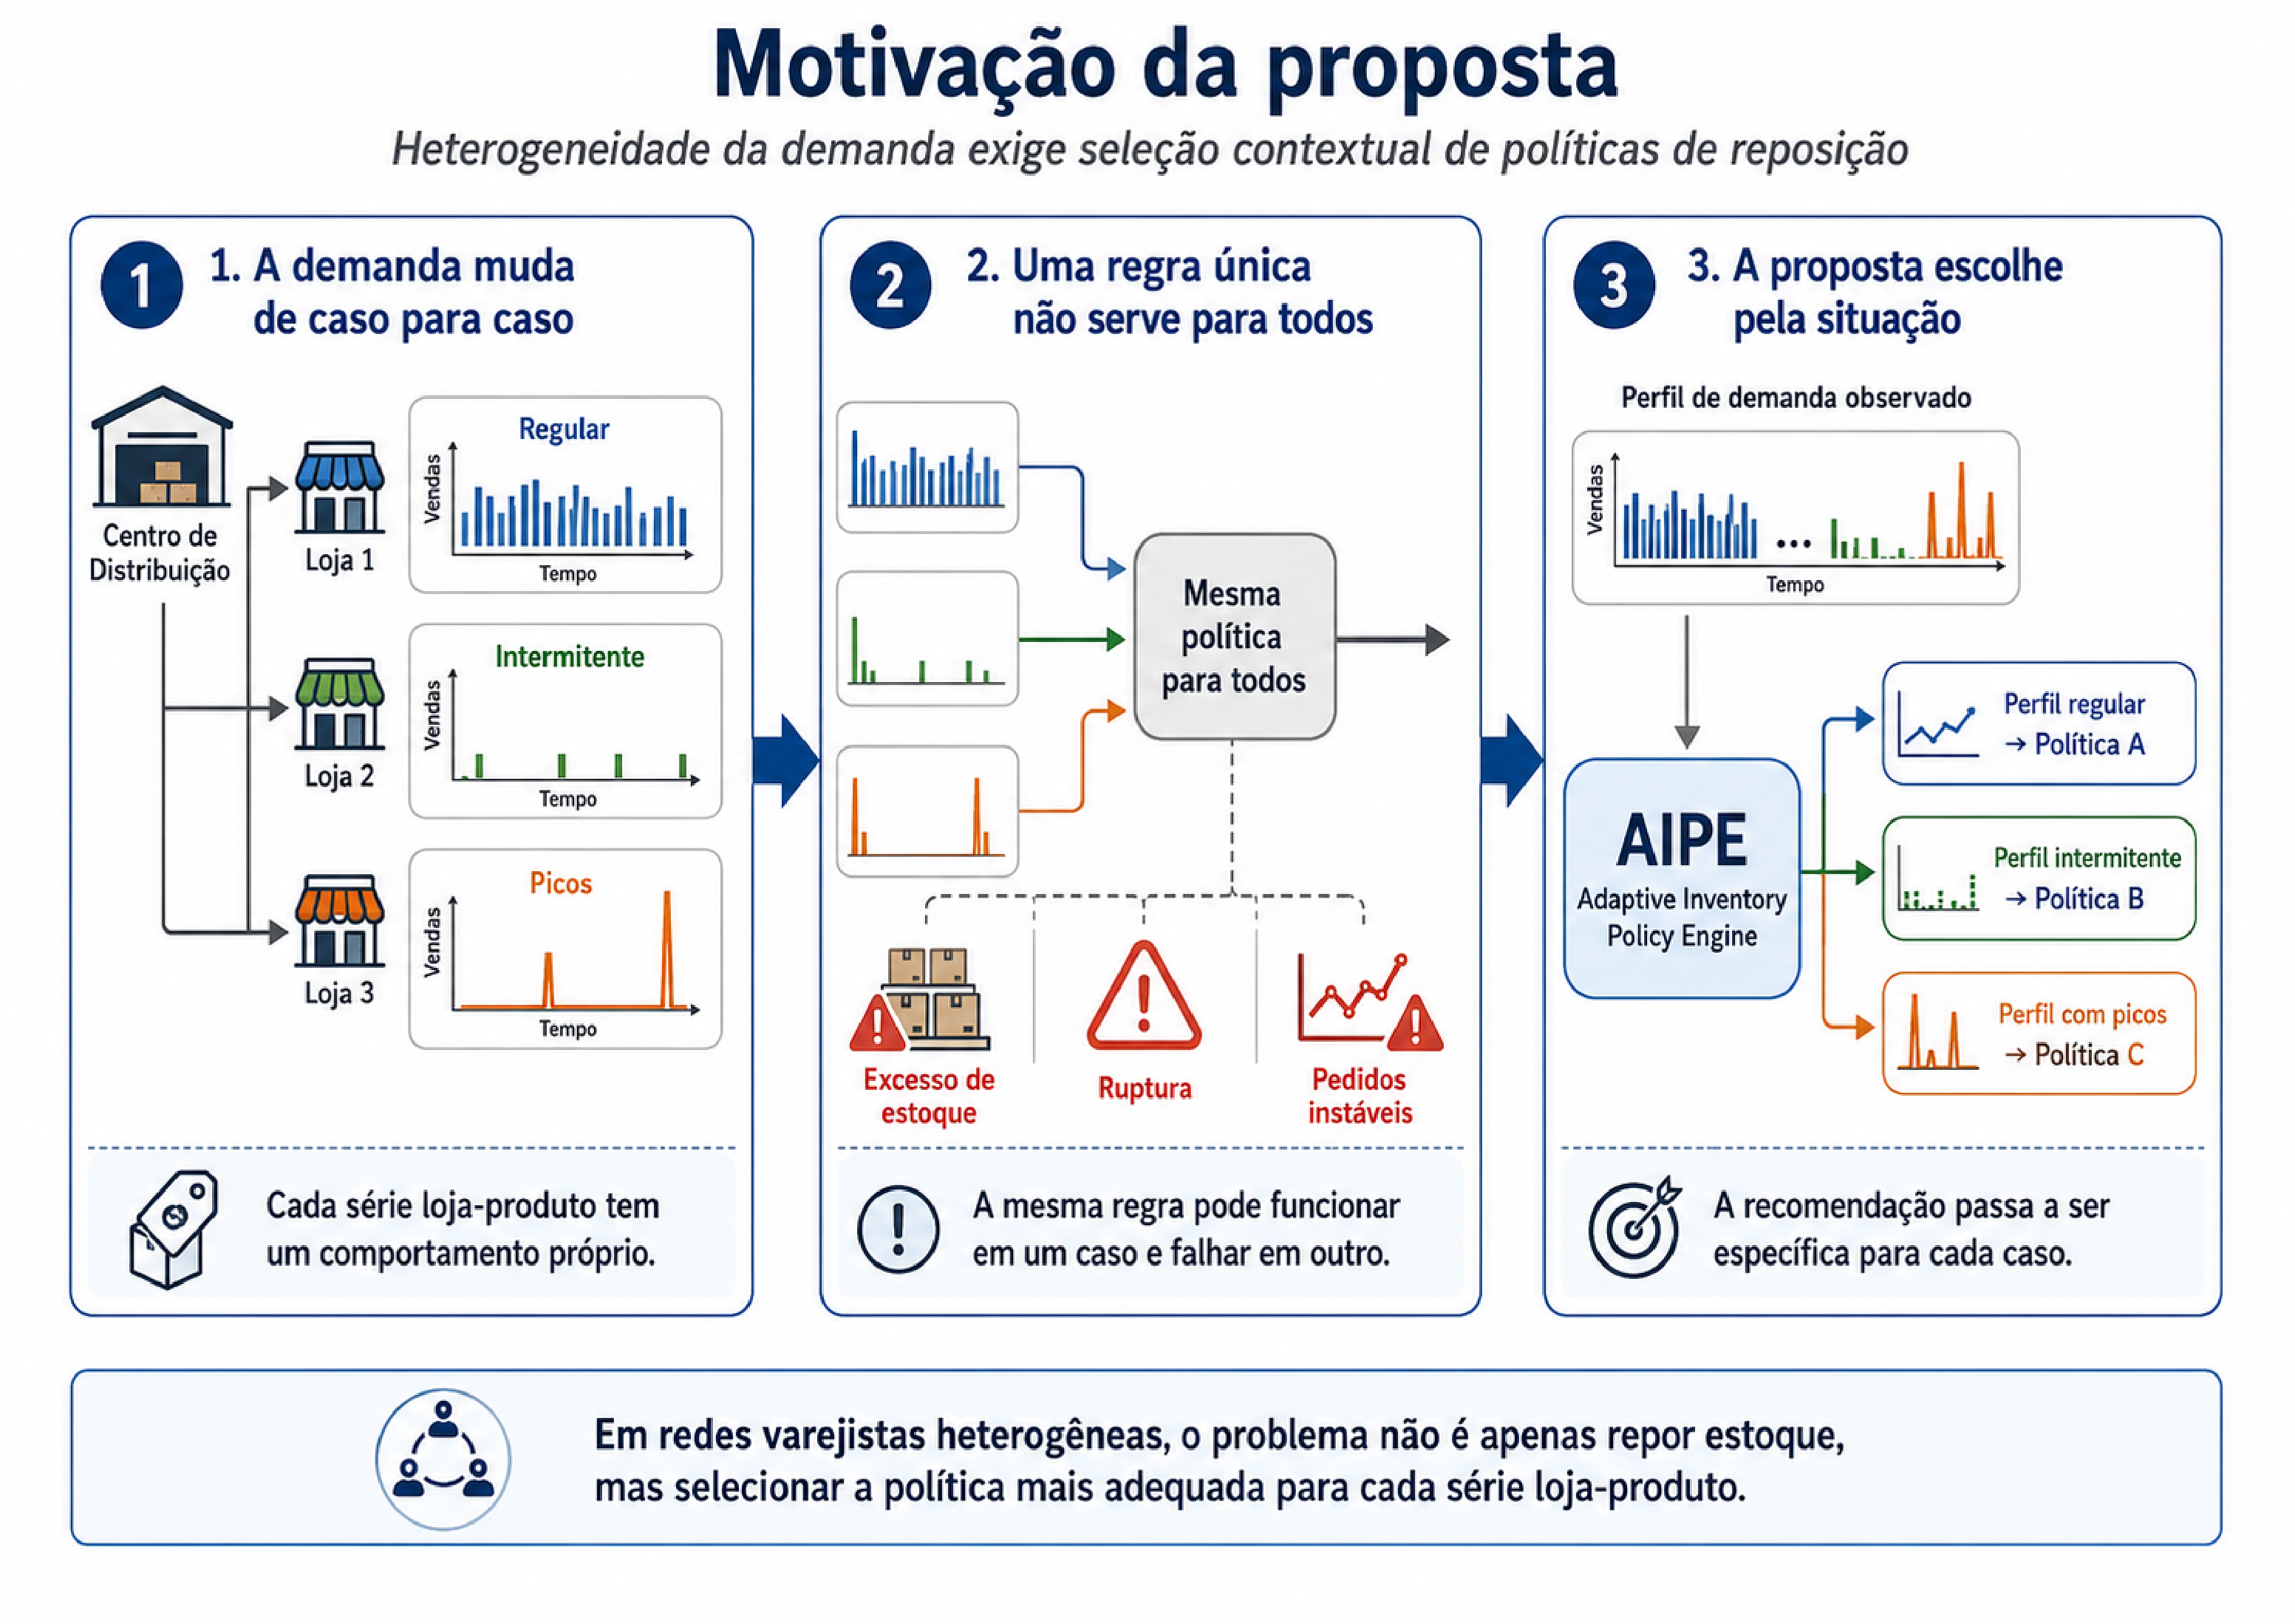
\includegraphics[width=\textwidth]{img/figura_1_1_motivacao_aipe.pdf}
\caption{Ilustra\c{c}\~ao conceitual da motiva\c{c}\~ao da disserta\c{c}\~ao. Em redes varejistas, diferentes s\'eries loja-produto podem apresentar vendas regulares, intermitentes ou concentradas em picos. A aplica\c{c}\~ao uniforme de uma mesma regra de reposi\c{c}\~ao pode gerar excesso de estoque, ruptura ou instabilidade nos pedidos. A proposta do AIPE \'e tratar essa diferen\c{c}a como um problema de sele\c{c}\~ao contextual de pol\'iticas de reposi\c{c}\~ao.}
\label{fig:intro_problem_selection}
\end{figure}
